% This version of CVPR template is provided by Ming-Ming Cheng.
% Please leave an issue if you found a bug:
% https://github.com/MCG-NKU/CVPR_Template.

\documentclass[final]{cvpr}

\usepackage{times}
\usepackage{epsfig}
\usepackage{graphicx}
\usepackage{amsmath}
\usepackage{amssymb}
\usepackage{graphicx}
\usepackage{caption}
\usepackage{dirtytalk}

% Include other packages here, before hyperref.

% If you comment hyperref and then uncomment it, you should delete
% egpaper.aux before re-running latex.  (Or just hit 'q' on the first latex
% run, let it finish, and you should be clear).
\usepackage[pagebackref=true,breaklinks=true,colorlinks,bookmarks=false]{hyperref}


\def\cvprPaperID{****} % *** Enter the CVPR Paper ID here
\def\confYear{CVPR 2021}
%\setcounter{page}{4321} % For final version only


\begin{document}

%%%%%%%%% TITLE
\title{Multi-Modal Depth Sensing}

\author{Robert Marcus\\
Carnegie Mellon University\\
{\tt\small rbm@cmu.edu}
% For a paper whose authors are all at the same institution,
% omit the following lines up until the closing ``}''.
% Additional authors and addresses can be added with ``\and'',
% just like the second author.
% To save space, use either the email address or home page, not both
%\and
%\\
%First line of institution2 address\\
{\tt\small}
}

\maketitle


%%%%%%%%% ABSTRACT
\begin{abstract}
	There are multitude of ways to compute a target objects depth by imaging. These methods, taken on their own, typically suffer some variety of drawbacks, ranging from low accuracy to high cost. Taken together, however, these methods can alleviate or greatly reduce the others deficiencies. We review an approach for combining LIDAR measured depth information with normals recovered by two methods - shape from polarization, and photometric stereo. Additional discussion is dedicated to a high level overview of methods for improving shape from polarization, and why these adjustments are merited.  
\end{abstract}

%%%%%%%%% BODY TEXT
\section{Introduction}

\subsection{Problem Background}
There are various methods for extracting the depth information of target objects. A number of methods have gained prominence in recent years. Some of these \textit{Shape-From-x} methods can be summarized briefly as follows: 
\begin{enumerate}
	\item Structured light
	\subitem Pros: Fast, high fidelity, precise.
	\subitem Cons: Expensive, useful implementations may be impractically large.
	\item Photometric stereo
	\subitem Pros: Allows re-rendering of an image, recovers additional useful properties.
	\subitem Cons: Requires many exposures, not useful for many materials, accuracy can be lacking.
	\item Stereo-vision
	\subitem Pros: Fast, uses commercial hardware
	\subitem Cons: High touch setup, scales poorly, accuracy is constrained by size of setup.
	\item Polarization
	\subitem Pros: Potentially fast, works with a variety of materials and lighting conditions
	\subitem Cons: Significant ambiguities during recovery lead to low accuracy.
\end{enumerate} 
On their own, each of these methods suffer from significant drawbacks. In general, it would be fair to say that \textit{shape-from-} stereo and polarization methods would benefit from the high precision of the structured light approach, and the structured light method would benefit from the compact size and economy of scale of the former. It has been shown, in fact, that while the underlying properties of each method cannot be reduced, by combining the methods at various points in the process of reconstructing an objects shape, superior results can be achieved than by each method on their own. 

That is, to say, we can use smaller, lower quality, and cheaper imaging solutions to achieve superior results by combining these multiple modes of sensing to build our reconstruction. This has the effect of mitigating specific drawbacks of individual methods on their own. 

For example, say we wanted to construct a device for scanning vases of variable material. We could, for example, choose to use a structured light approach with a laser scanner, i.e., an Intel L515 LiDAR. However, at its best, the L515 has a 5mm spatial resolution, which may be insufficiently \textit{accurate} for the task. Alternatively, we could try using photometric stereo to achieve our goal, however, due to material variability, lighting imperfections, etc., this approach may be insufficiently \textit{precise} without post-processing. The same could be said, for example, by undertaking a shape from polarization approach.

It would be convenient if we could combine the methods in such a way that we could keep the high accuracy of the visual methods with the high precision of the structured light method. 

\subsection{Problem Approach}

It has been shown by Nehab Et Al that we can perform this operation on aligned datasets \cite{NehabSource}. Specifically, given we have the normals of an object, and a depth map aligned to the perspective of those normals, we can combine them in such a way that combines the high-frequency details of the visual image with the precision of depth maps. 

In other words, for a given scene, we can loosely state an approach to this problem as follows: 
\begin{enumerate}
	\item Collect our depth map by structured light (LIDAR, TOF, etc.)
	\item Collect our images by some procedure\footnote{In this paper, we consider photometric stereo and shape from polarization.}.
	\item Align the requisite data.
	\item Construct our normals and pre-process to correct for ambiguities
	\subitem In the case of shape from polarization, we can involve the depth map to constrain the ambiguities in the normals, as shown by Kadambi Et Al \cite{Kadambi2017}.  
	\item Construct a new depth map by combining the depth map and normals following the procedure outlined by Nehab et al, giving the depth map weight $\lambda$, and the normals weight $1 - \lambda$.
\end{enumerate}
We will discuss each step in the following methods sections, preceded by giving a minor recap of uncalibrated photometric stereo, as well as a gentle introduction to shape from polarization. 

\section{Method}
\subsection{Collecting and aligning the depth map and image frames.}
This project was centered around the usage of an Intel L515 Realsense depth sensing camera. It features a LIDAR sensor which can be used to stream depth and color RGB information simultaneously. Interfacing with the unit is handled by the \href{https://intelrealsense.github.io/librealsense/python_docs/_generated/pyrealsense2.html}{PyRealsense2 Python API}\footnote{Note, as of writing this, the PyRealsense2 library is essentially only usable on Windows. Installing this on MacOS, and, especially ARM MacOS, is a futile exercise.}.

The setup for this experiment featured placing the L515 on a tripod, approximately one meter away from the target scene, where the units spatial resolution is maximized (about 5mm.) We are able to mask out the scenes foreground and background using the devices depth range to build a binary mask of all pixels within a certain range. 

Additionally, the device camera and LIDAR sensor were aligned using the cameras intrinsic information, which is made available through the PyRealsense2 API. See figure 1 at the end of the document for a reference of the setup. 

One limitation of this method is that the L515 is not natively capable of capturing RAW image information \footnote{It is, interestingly, capable of capturing raw depth map information.}. This presents a challenge for photometric stereo, as preferably we would pass in linearized \verb|tiff| images. We settle by using linearized PNG's, where each image has been gamma-corrected by the following map: 
$$I_{\text{lin}}(I_{\text{nl}}) = \begin{cases}
	\frac{I_{\text{nl}}}{12.92} & I_{\text{nl}} \leq 0.0404482 \\
	\left(\frac{I_{\text{nl}}+0.055}{1.055}\right)^2.4 & \text{o.w}
\end{cases}$$
\begin{figure}
	\begin{minipage}[b]{0.4\textwidth}
		\centering
		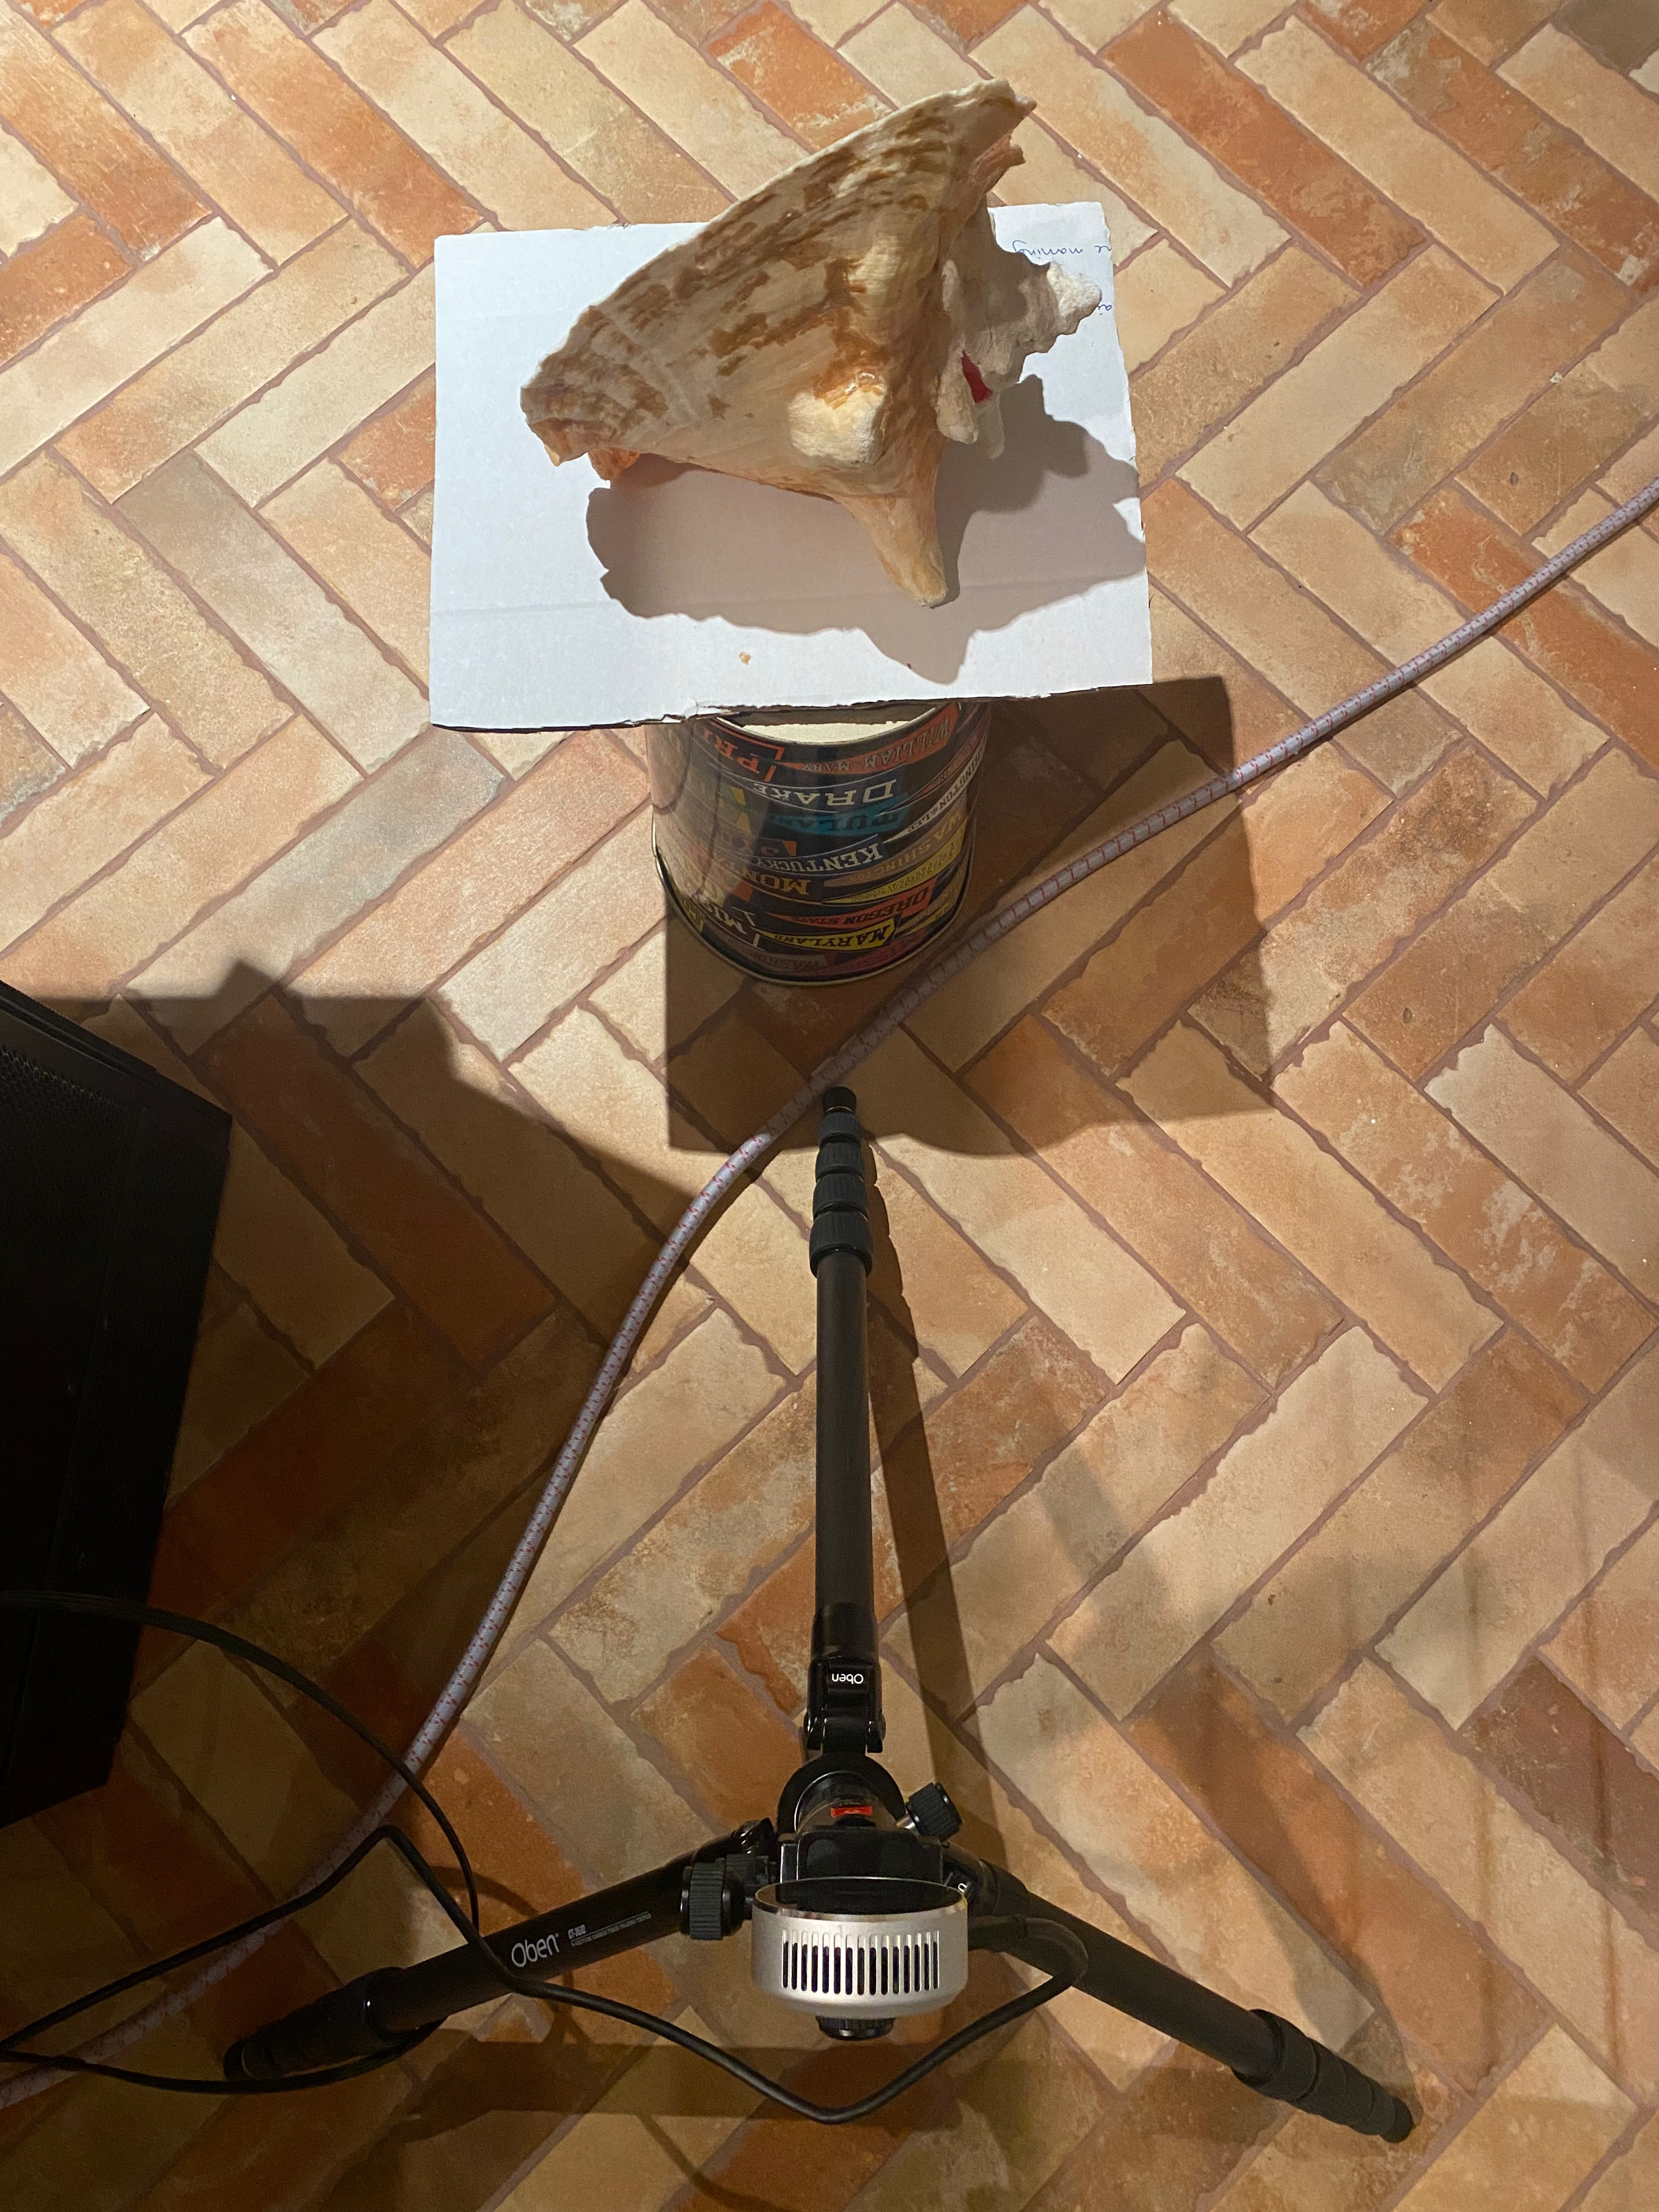
\includegraphics[width=6cm]{experimental_setup}
		\captionof{figure}{
		The experimental setup. When dealing with SfP, a 55m circularly polarized filter is placed on the front surface of unit.
		}
	\end{minipage}
\end{figure}

\subsection{Constructing normals}
\subsubsection{Constructing normals by uncalibrated photometric stereo}
For context on this approach, see homework 5 from 15-463.
\subsubsection{Constructing normals by SfP}
\begin{figure}
	\centering
	\includegraphics[width=7cm]{sfp_diagram}	
	\caption{The basic scheme of SfP. It becomes clear how we can reconstruct the normals by going from spherical coordinates to cartesian.}
\end{figure}

	There are several different approaches for constructing normals by SfP. We follow the approach laid out by Smith Et al in \textit{Linear depth estimation from an uncalibrated, monocular polarisation image}, which makes the assumptions that the ambient light is unpolarized, the materials are dielectric, and surfaces are specular dominant. We have tried our best to follow these assumptions with our scene, using what we believe to be a polarized filter in between the scene and the sole point light source. 
	
	We additionally assume a fixed refraction index of $n=1.5$ for simplicity, and because it is approximately average for the given restrictions.
	
	
	We will now establish the math needed to go from raw images to normals, which is fairly straightforward to lay out from a high level\footnote{Which is not to say it is easy to implement in practical terms.} The two terms we would like are the zenith ($\theta$, the reflection angle off the surface) and azimuth ($\phi$, the phase angle of the reflected ray.) 
	
	We can parametrize every pixel in the image by three quantities, its phase $\phi$, the degree of polarization $\rho$, and the unpolarized intensity, $i_{\text{un}}$. 
	
	Principally, we must capture multiple images of the scene to parameterize the sinusoid characterizing the intensity of the pixels across filter rotations. We calculated the phase angle using a non-linear curve fitting approach for a given pixel $p_{x,y}$ across the various filtering rotations. 
	
	Additionally, the degree of polarization $\phi$ can be taken as $\phi = \frac{I_{\max} - I_{min}}{I_{\max} + I_{\min}}$, and our unpolarized intensity $i_{\text{un}}$ can be taken as $i_{\text{un}} = \frac{I_{\max} + I_{\min}}{2}$\footnote{The unpolarized intensities can be used to enforce additional surface normal constraints by assuming light is reflected according to the Lambertian model. We do not implement this constraint, but the value is explicated for consistency with general SfP explanations.}
	
	We can relate the zenith $\theta$ to the degree of polarization by Fresnels equations, namely, 
	
	$$\rho = \frac{(n - \frac{1}{n})^2 \sin\theta}{4 \cos\theta \sqrt{n^2 - \sin^2\theta} - \sin^2\theta (n + \frac{1}{n})^2 + 2n^2 + 2}$$Where $\rho, n$ are both known, and we can solve for $\theta$ by any number of manners. We choose to solve for it directly using a procedure outlined by Kadambi \cite{Kadambi2017}. Note though that this is where a key ambiguity is introduced in SfP - both $\theta$, and $\theta + \pi$ are solution to the above. We can correct for this ambiguity in practice, either by disamb
	
	By recovering $\phi, \theta$, we can then translate our parametrization into a cartesian normals by $$n = \begin{bmatrix}
		\sin\phi \sin\theta\\
		\cos\phi \sin\theta\\
		\cos \theta
	\end{bmatrix}$$
	
	The above procedure should theoretically yield the relevant surface normals. However, in practice, these efforts are beguiled by three physical constraints, as noted in Kadambi \cite{Kadambi2017}:
	\begin{enumerate}
		\item Azimuthal ambiguity (as noted above)
		\item Refractive unknowns
		\subitem the $n=1.5$ assumption is inexact and leads to inaccuracies. It is rarely practical to know the refractive index at every pixel in the scene.
		\item Fronto parallel surfaces
		\subitem When the zenith angle is near zero, the obtained normals are noisy\footnote{This is evident in my data, in figure 3 and 4, with the foam roller.}  
	\end{enumerate} 
	
	
\subsection{Combining positions and normals}
	Nehab et al formulated the question of finding an optimal surface in terms of a minimization problem regarding two error terms - that of the depth measurements, $E^p$, and the normal measurements, $E^n$: $\text{argmin}_{Z} \lambda E^p + (1 - \lambda) E^n$. Here, $\lambda \in [0, 1]$ is a weight controlling how much of the fused output should consist of the normals versus the depth.
	
	Nehab provides a formulation of the minimization problem that relies on surface tangents of the depth map. These tangents can be written as linear in terms of the depth. We rely on Yu et al \cite{InverseRenderingYuSmithNehabMethod} for an explicit formulation of this minimization problem, whereby our tangent vectors can rather artfully be laid out as follows:
	\begin{align*}
		T_x = \begin{bmatrix}-\frac{1}{f_x}X & -\frac{1}{f_x}I\\-\frac{1}{f_y}Y & 0\\
		I & 0\end{bmatrix}\begin{bmatrix}\frac{\partial Z}{\partial x}\\
		I\end{bmatrix}	&  & T_Y = \begin{bmatrix}-\frac{1}{f_x}X & 0\\-\frac{1}{f_y}Y & -\frac{1}{f_y}I\\
		I & 0\end{bmatrix}\begin{bmatrix}\frac{\partial Z}{\partial y}\\
		I\end{bmatrix}
	\end{align*}
	Where $X, Y$ form a meshgrid over the $N \times M$ size image, and $I, 0$ are the relevant matrices of the same size. As constructed in code, these form a highly sparse matrix of size $NM \times NM$. Additionally, $f_x, f_y$ are the respective axis focal lengths of the camera in pixels, retrieved with the other camera intrinsics during the alignment step. 
	
	Each pixel in the image yields 3 equations or less: one equation for the position error. This allows us to solve the system by least squares as it is highly overconstrained. To that end, we similarly build a very sparse representation of the normals so we can incorporate them into the minimization, building them as the $NM \times 3NM$ matrix containing the channelwise normals. We are left to solve the over-constrained least squares problem of $\begin{bmatrix}\lambda I\\NT_x\\NT_y\end{bmatrix} \hat{z} = \begin{bmatrix}z\\
	0\\
	0 \end{bmatrix}$ where the left hand side has shape $3NM \times NM$ $z$ is our flattened depth map of size $1 \times NM$, and each $0$ is the $1\times NM$-sized 0-vector. This can be solved rather easily, and gives us the $NM$-length vector $\hat{z}$ containing the optimal depth surface. 
	This procedure works as the surface is effectively minimized by the tangents being made perpendicular to the corrected normals, i.e., their dot product is zero. 

\section{Results}
\begin{figure*}
	\begin{center}
	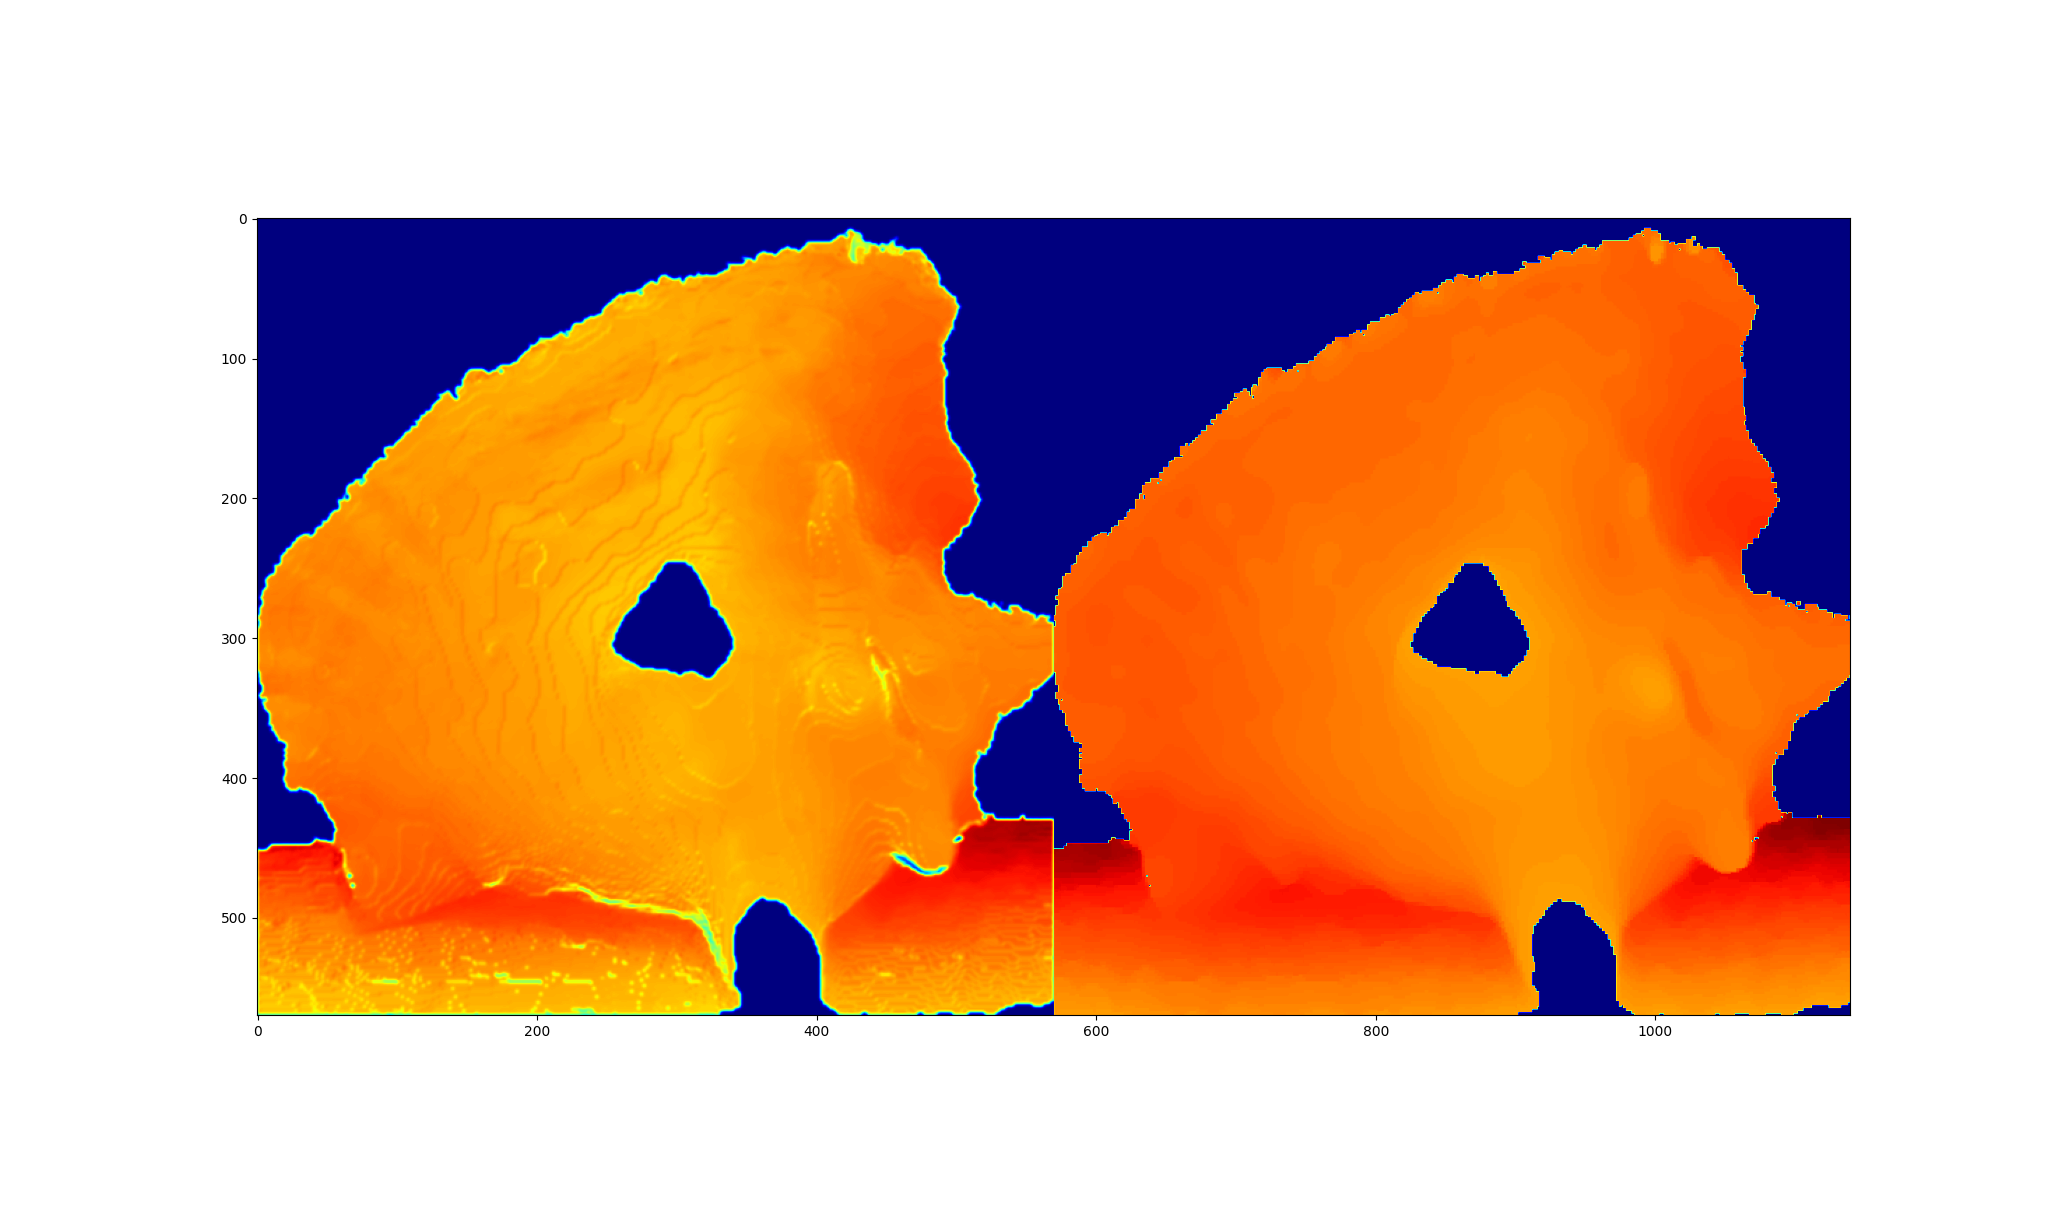
\includegraphics[width=10cm]{ps_conch}
	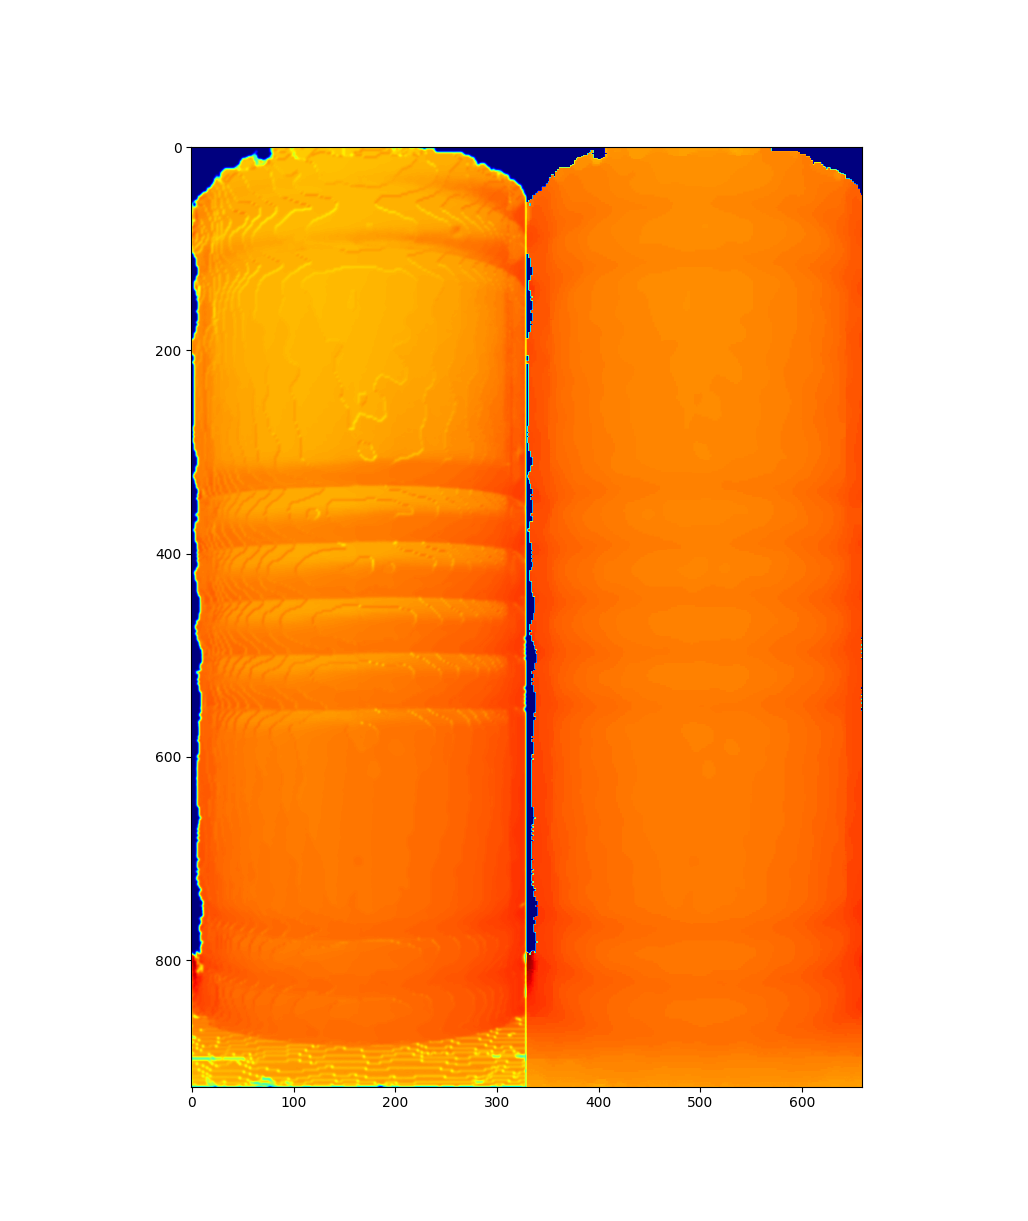
\includegraphics[width=5cm]{ps_roller}
	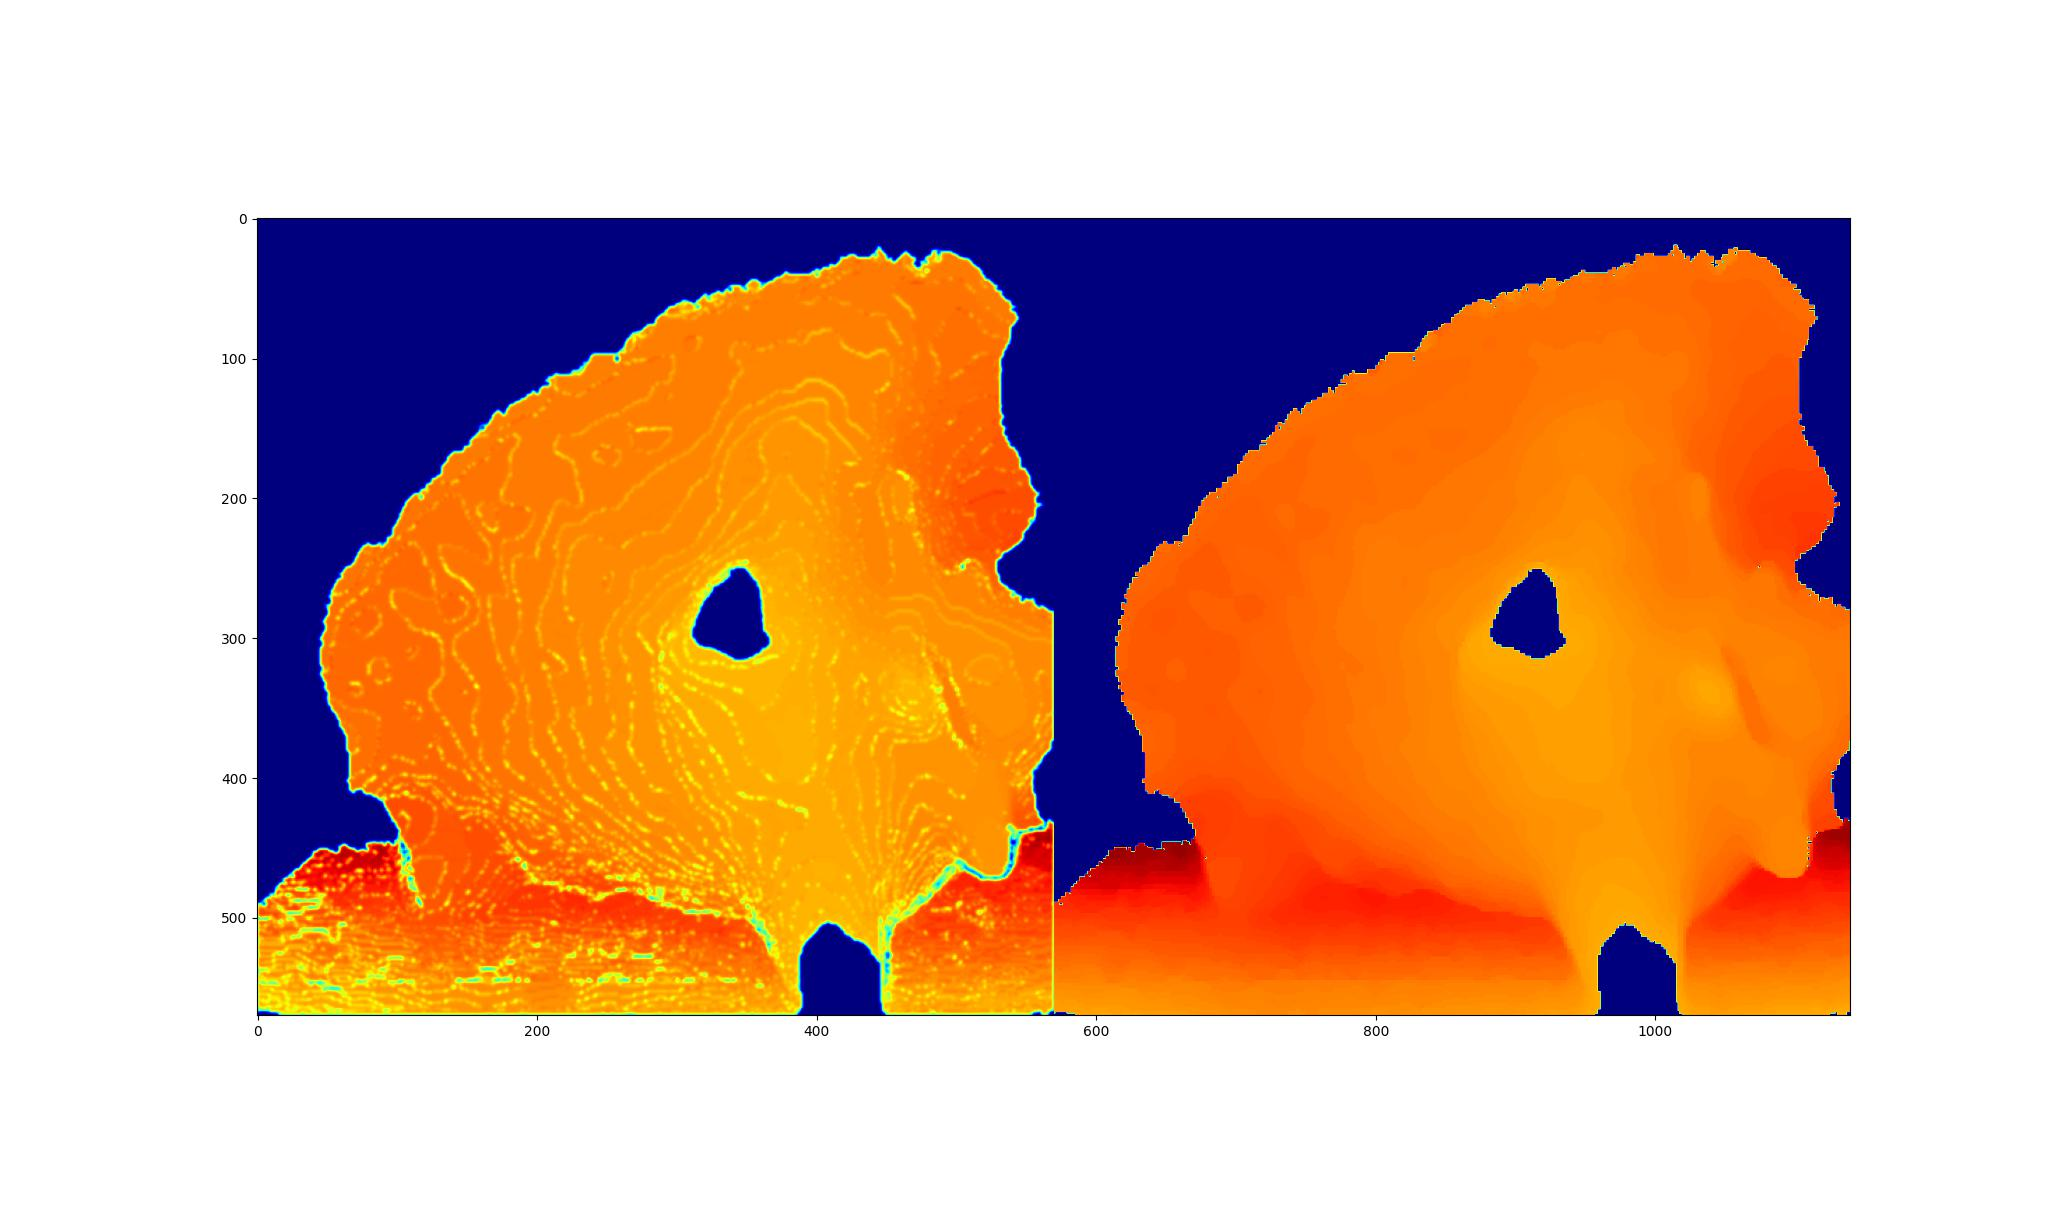
\includegraphics[width=10cm]{sfp_conch}
	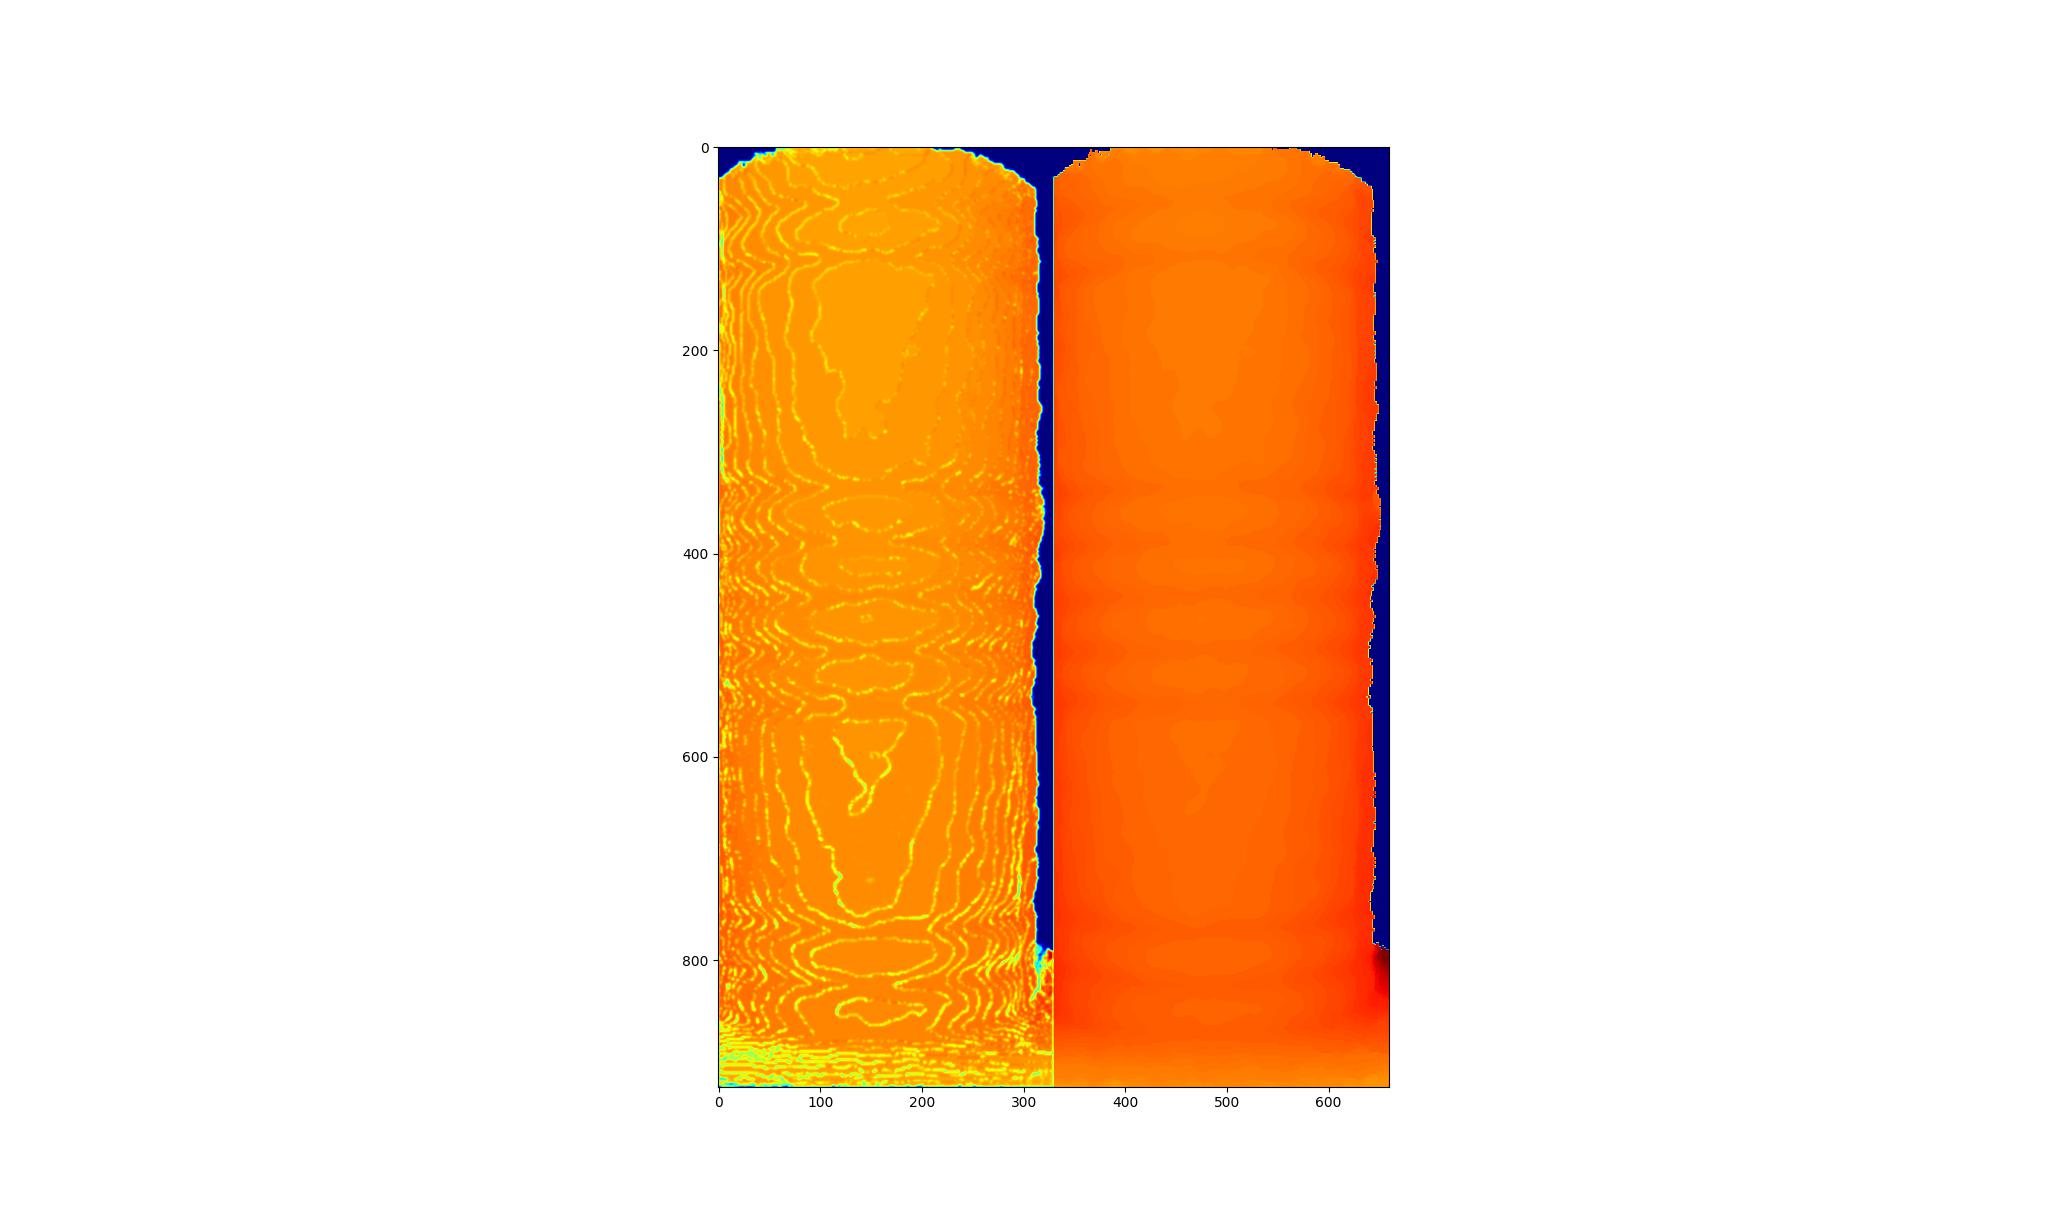
\includegraphics[width=5cm]{sfp_roller}
	\caption{The improvements from the merging algorithm on the left versus the original depth maps on the right. On the top, results from the photometric stereo normals. On the bottom, results from the polarization normals.}	
	\end{center}
\end{figure*}

\begin{figure*}
	\begin{center}
		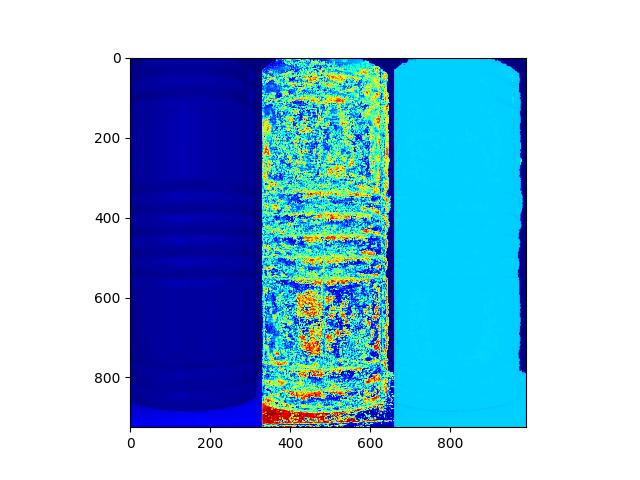
\includegraphics[width=8cm]{sfp_roller_parametrization.jpeg}
		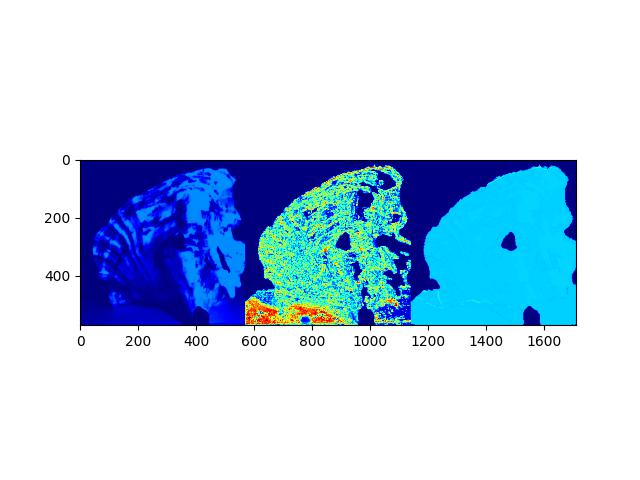
\includegraphics[width=10cm]{sfp_conch_parameterization}
		\caption{The intensities, the azimuth angles, and the zenith angles of the polarized photos.} 
	\end{center}	
\end{figure*}

We captured four sets of data of two Lambertian objects for this data. Two sets of polarized data, where 4 frames were captured of the object with a linear polarizer in front of the L515 unit, rotated at the angles $0^{\circ}, 45^{\circ}, 90^{\circ}, 135^{\circ}$\footnote{The polarizer angle was calibrated to $0^{\circ}$ by rotating it in front of a polarizing light source until the light passing through the filter was at its brightest. A ring of paper was taped around the filter and the relevant points were marked on the filter in this manner.}.  

See figure 3 and 4 at the end of the document for reference. 

Also provided are the recovered depolarized light intensities, the azimuth angles, and the zenith angles. Note these have not been processed for ambiguities as described by Kadambi \cite{Kadambi2017} (with respect to correcting azimuthal ambiguity, refractive distortions, or enforcing physics constraints through integration)  or Atkinson \cite{atkinson} (with respect to azimuthal disambiguation.) 

\section{Discussion}
The results from the photometric stereo data was excellent. The improvements are visually discernible on both datasets, with no obvious artifacts or degradations on the resultant depth maps. While the specific improvements are impossible to qualify because we lack a true ground source truth for the improvements, the results are certainly obvious in this context - in both cases, information that was entirely missing from the orignal depth map has now been incorporated, without distorting the map or introducing additional ambiguities. The results are impressive. 

However, this project was originally not focused on photometric stereo, and it's now obvious to the reader as to why the project has been extended to include it - the results with SfP are less than stellar. While the initial plan for this project included going far beyond naive SfP, unexpected friction was encountered from the very beginning. These headwinds meant that instead of delivering an optimized SfP with ambiguity improvements, instead we primarily have a slightly buggy naive SfP that isn't quite right. Notice the white contour lines on the conch or foam roller, for example. 

These contour lines correspond to sharp drops in the depth map that are certainly not present in the real scene. 

While the photometric stereo approach improved the depth map without introducing artifacts, the SfP approach introduced  artifacting to the depth map, for seemingly every value of $\lambda$. This is indicative of a normal map that is wrong in a kind of way. 

There are several possible explanations for this. One is that the data was improperly collected, which is possible - the angle calibrations on the circular filter were not exact, and, while we tried our best to place the filter at the right angular orientation for each capture, we could not have been exact. Additionally, the L515 was not designed for use with a polarizing filter, so it's possible the additional glass between the built in camera introduced too much additional distortion for the results to ever be meaningful. Finally, there is always the possibility for buggy code. Part of the issue here is that there are many different implements of "basic" normal recovery by SfP, each with their own minute differences in material and lighting assumption. This paper took the approach of Smith et al 2016 with \textit{Linear Depth Estimation from an Uncalibrated,  Monocular Polarisation Image} \cite{SmithSfPMath} as discussed in the method section. 

It's possible that we would have been better served by an approach that made fewer assumptions about the scene. However, we likely would have been stymied by the above physical limitations with respect to equipment either way. 

Additionally, even with a more successful SfP implementation, forward progress on resolving SfP ambiguities was somewhat unlikely. Kadambi undersells the difficulty of his approach, at least for those replicating his approach in modern Python - while there have historical been graphical model libraries in python, they are not readily available anymore, or we have not found the right libraries\footnote{For example, we came across old sources for the OpenGM library while designing an approach to handle section 4 of Kadambi, but were unable to build the library successfully after a day of trying. This meant large parts of Kadambi were essentially impractical to re-implement without significant additional effort.}. Similarly, when we tried implementing Atkinson's \cite{atkinson} disambiguation protocol in an attempt to improve the normals, we were stymied by debugging difficulties. Implementing the algorithm was difficult for all the normal reasons: the paper was less explicit than desired, the algorithm was quite slow, and debugging was difficult because it was hard to tell if the problem was bad data or bad design. In general,  experiments with SfP are not something the author would recommend undertaking in the future, and, perhaps they should have heeded Kadambi's warning on the practicality of SfP without additional processing steps: \say{Due to the limitations of SfP, SfP has never been considered as a robust alternative to SfS or PS.} 

In other words, the originally scoped project had a far greater all-or-nothing element to it than anticipated. 

Regardless, the results from re-implementing Nehab were quite good, and, given the limitations of naive SfP as discussed in methods section, the given results were fairly OK.  
\section{Material}
Data for this project is available at \href{https://github.com/rob-marcus/463-final-project}{the following github repository.} Additionally, almost all of the code for this project is available there as well, however, the uncalibrated photometric stereo code has not been released. The code largely contains citations where relevant, but some may be missing due to accidental oversight. See the relevant \verb|*_runner.py| code for usage and examples. 

\begin{figure}
\centering
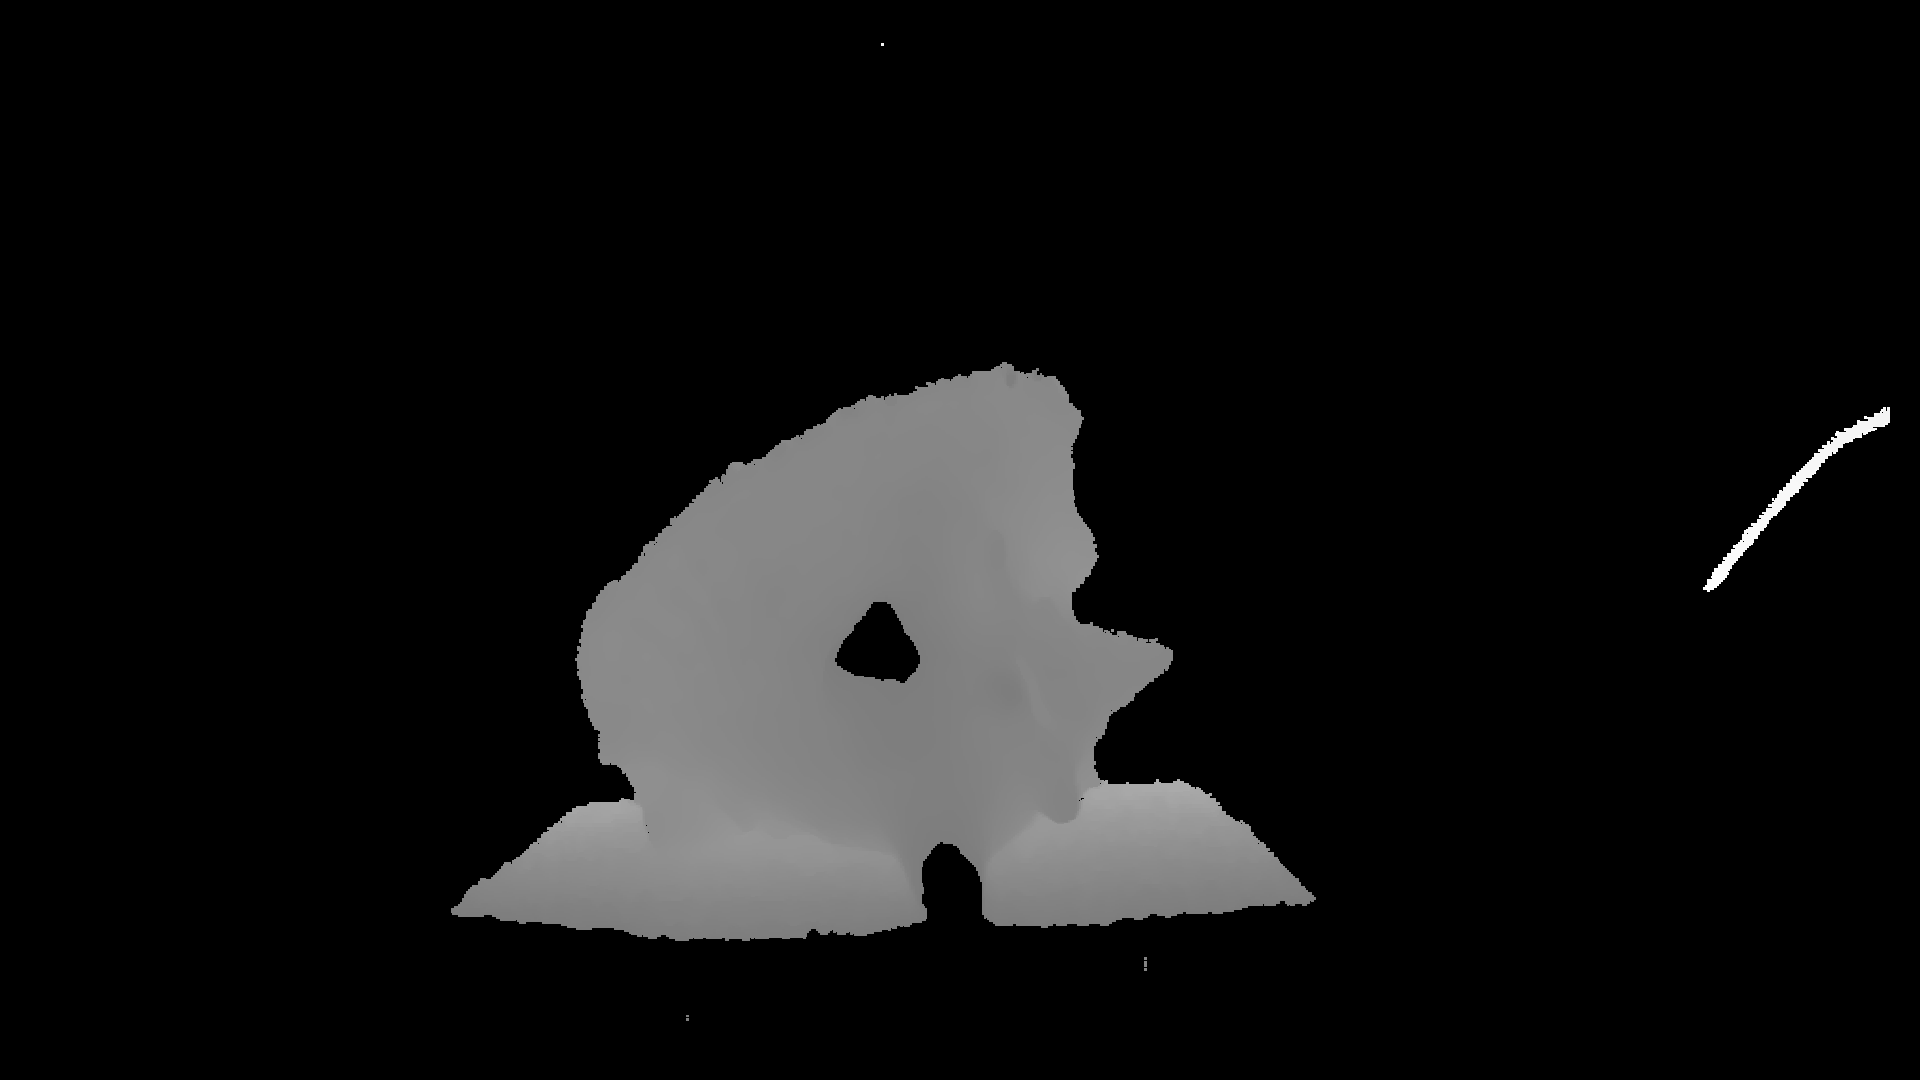
\includegraphics[width=8cm]{conch_depth_frame_sample}
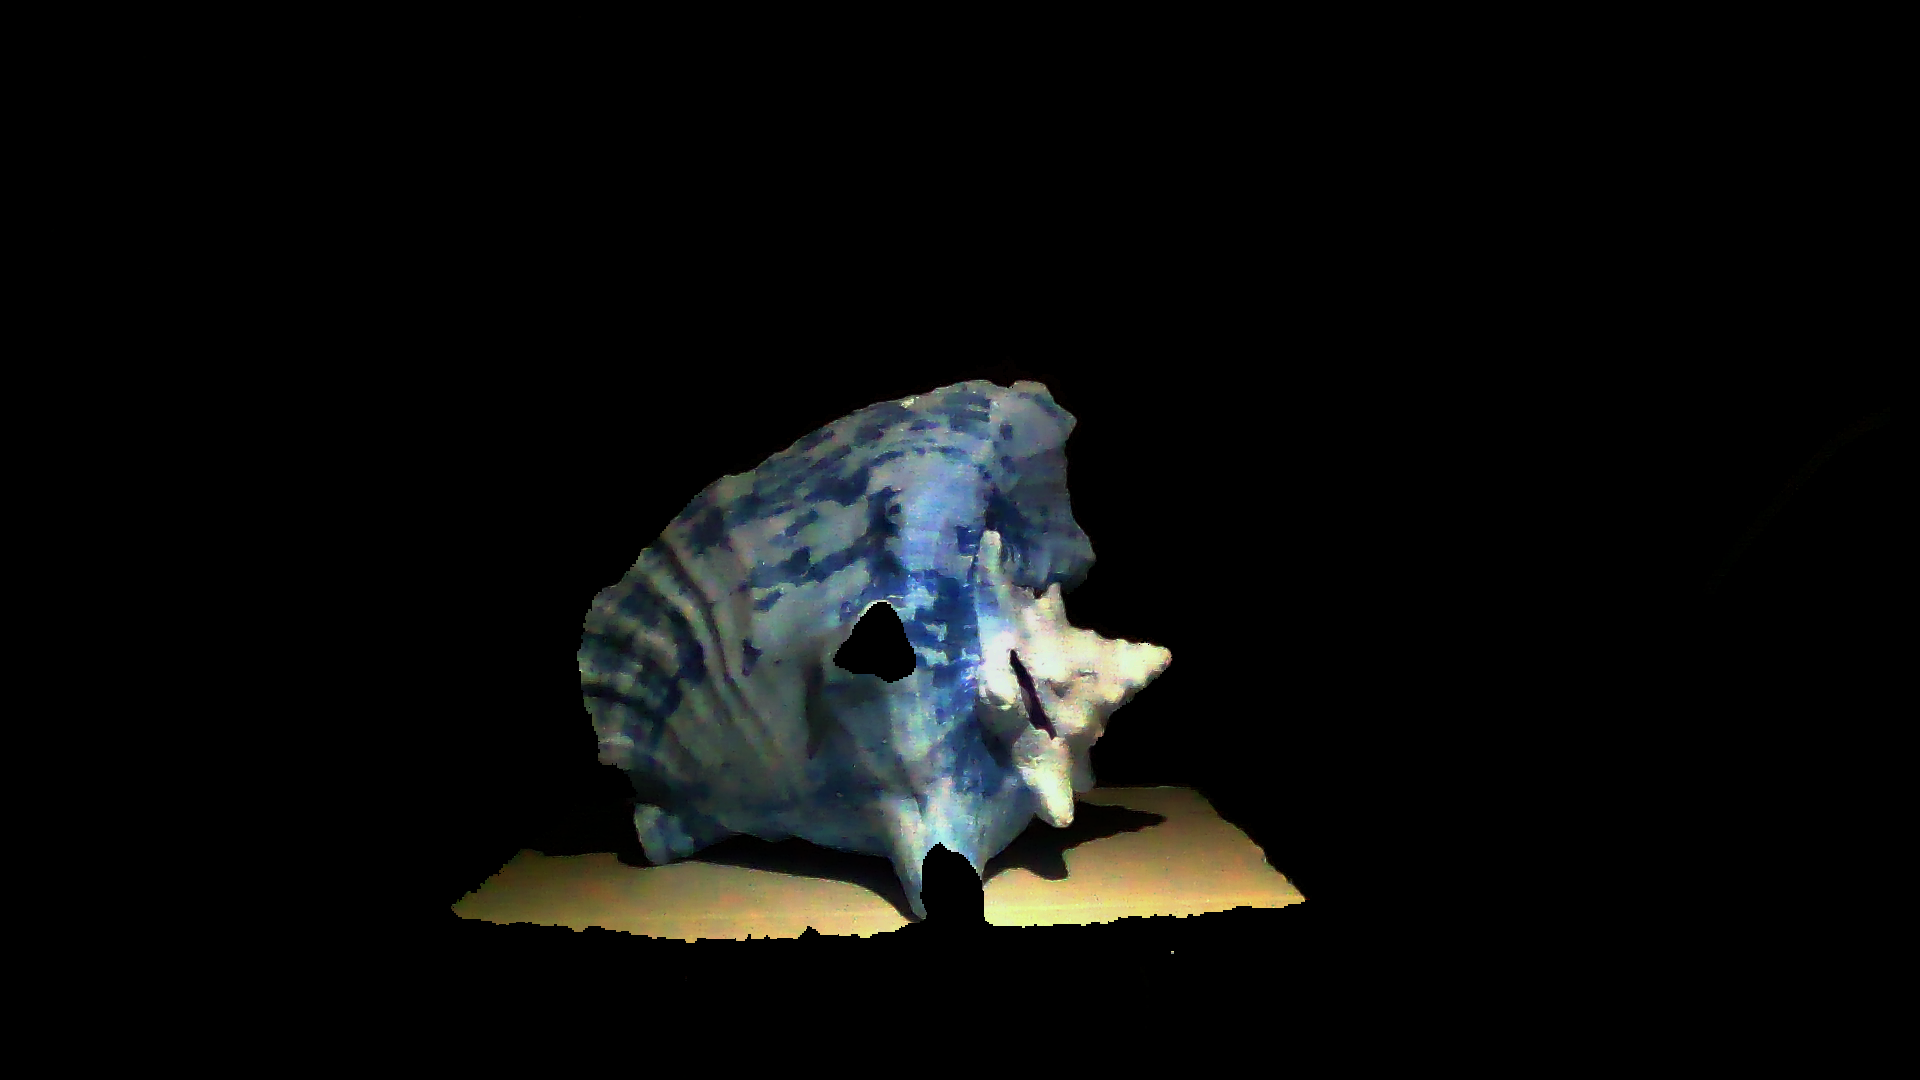
\includegraphics[width=8cm]{conch_sample}
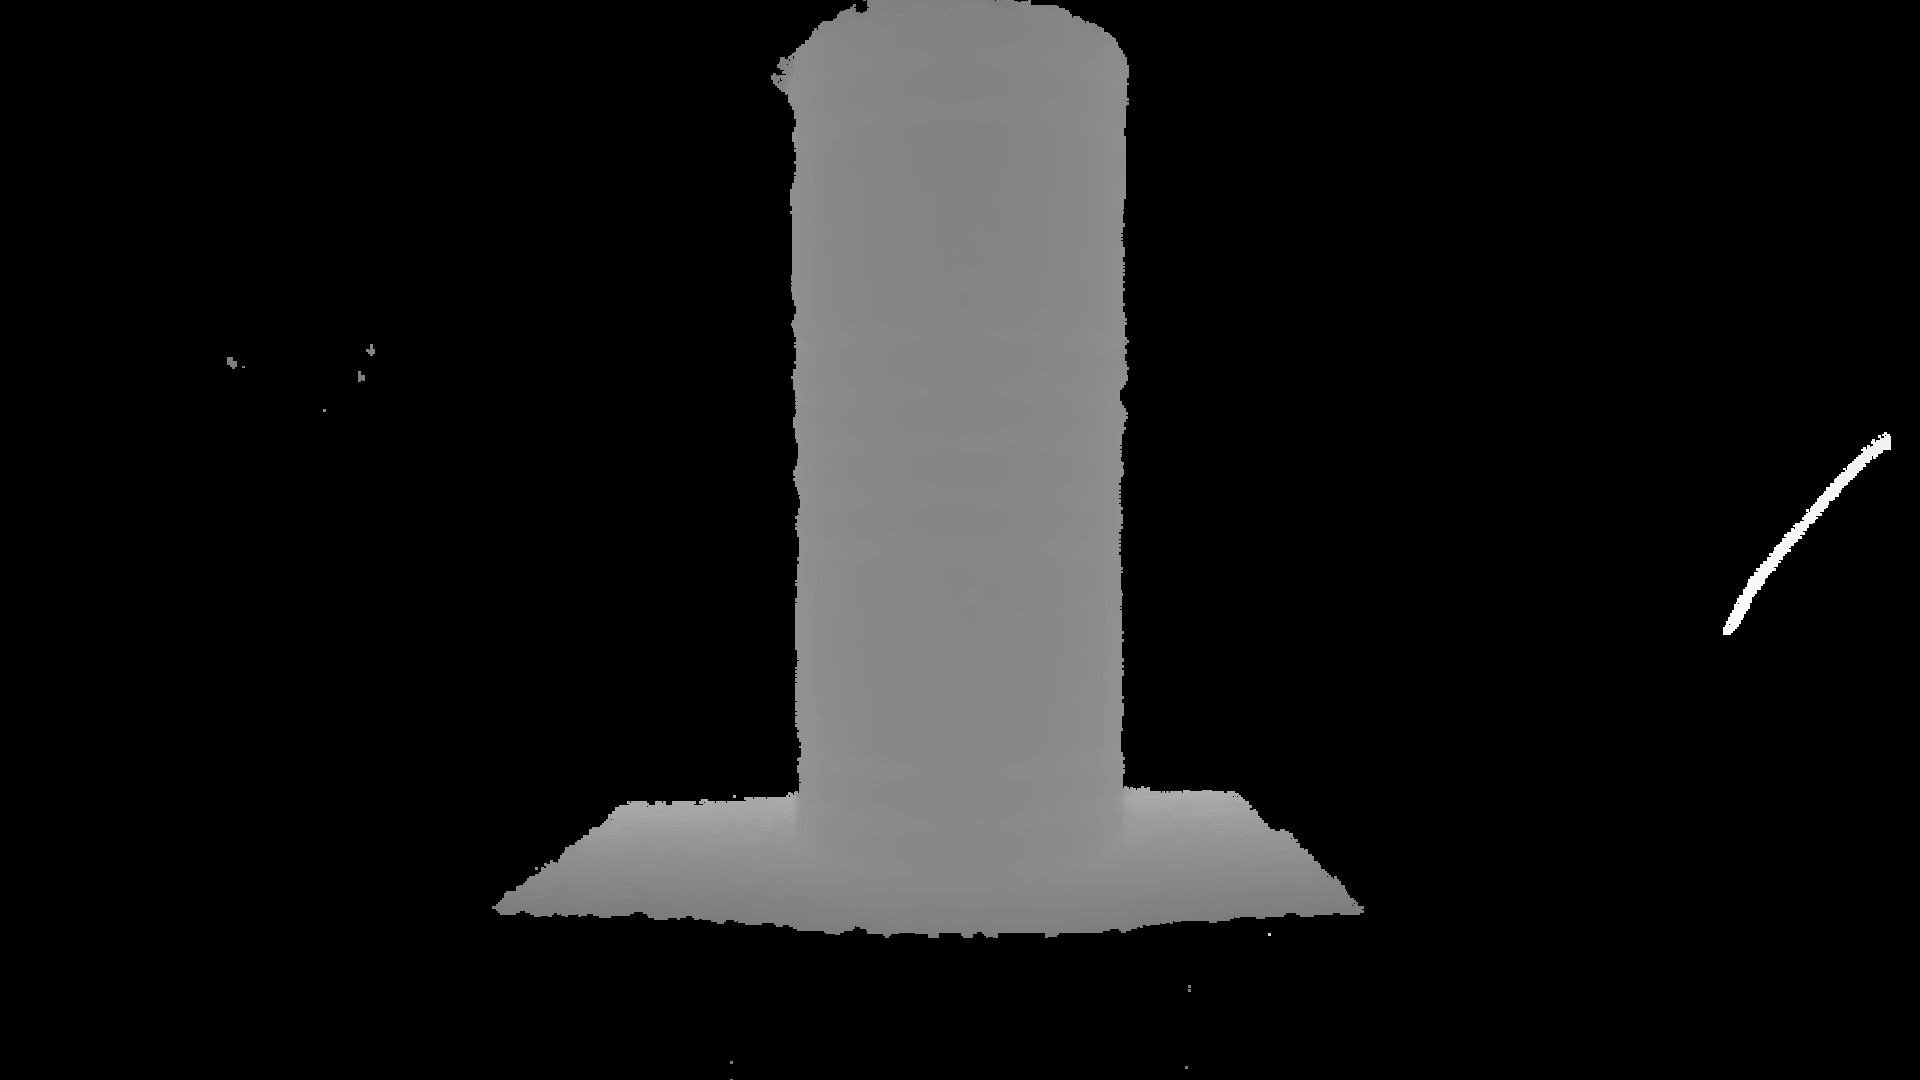
\includegraphics[width=8cm]{roller_depth_frame_sample}
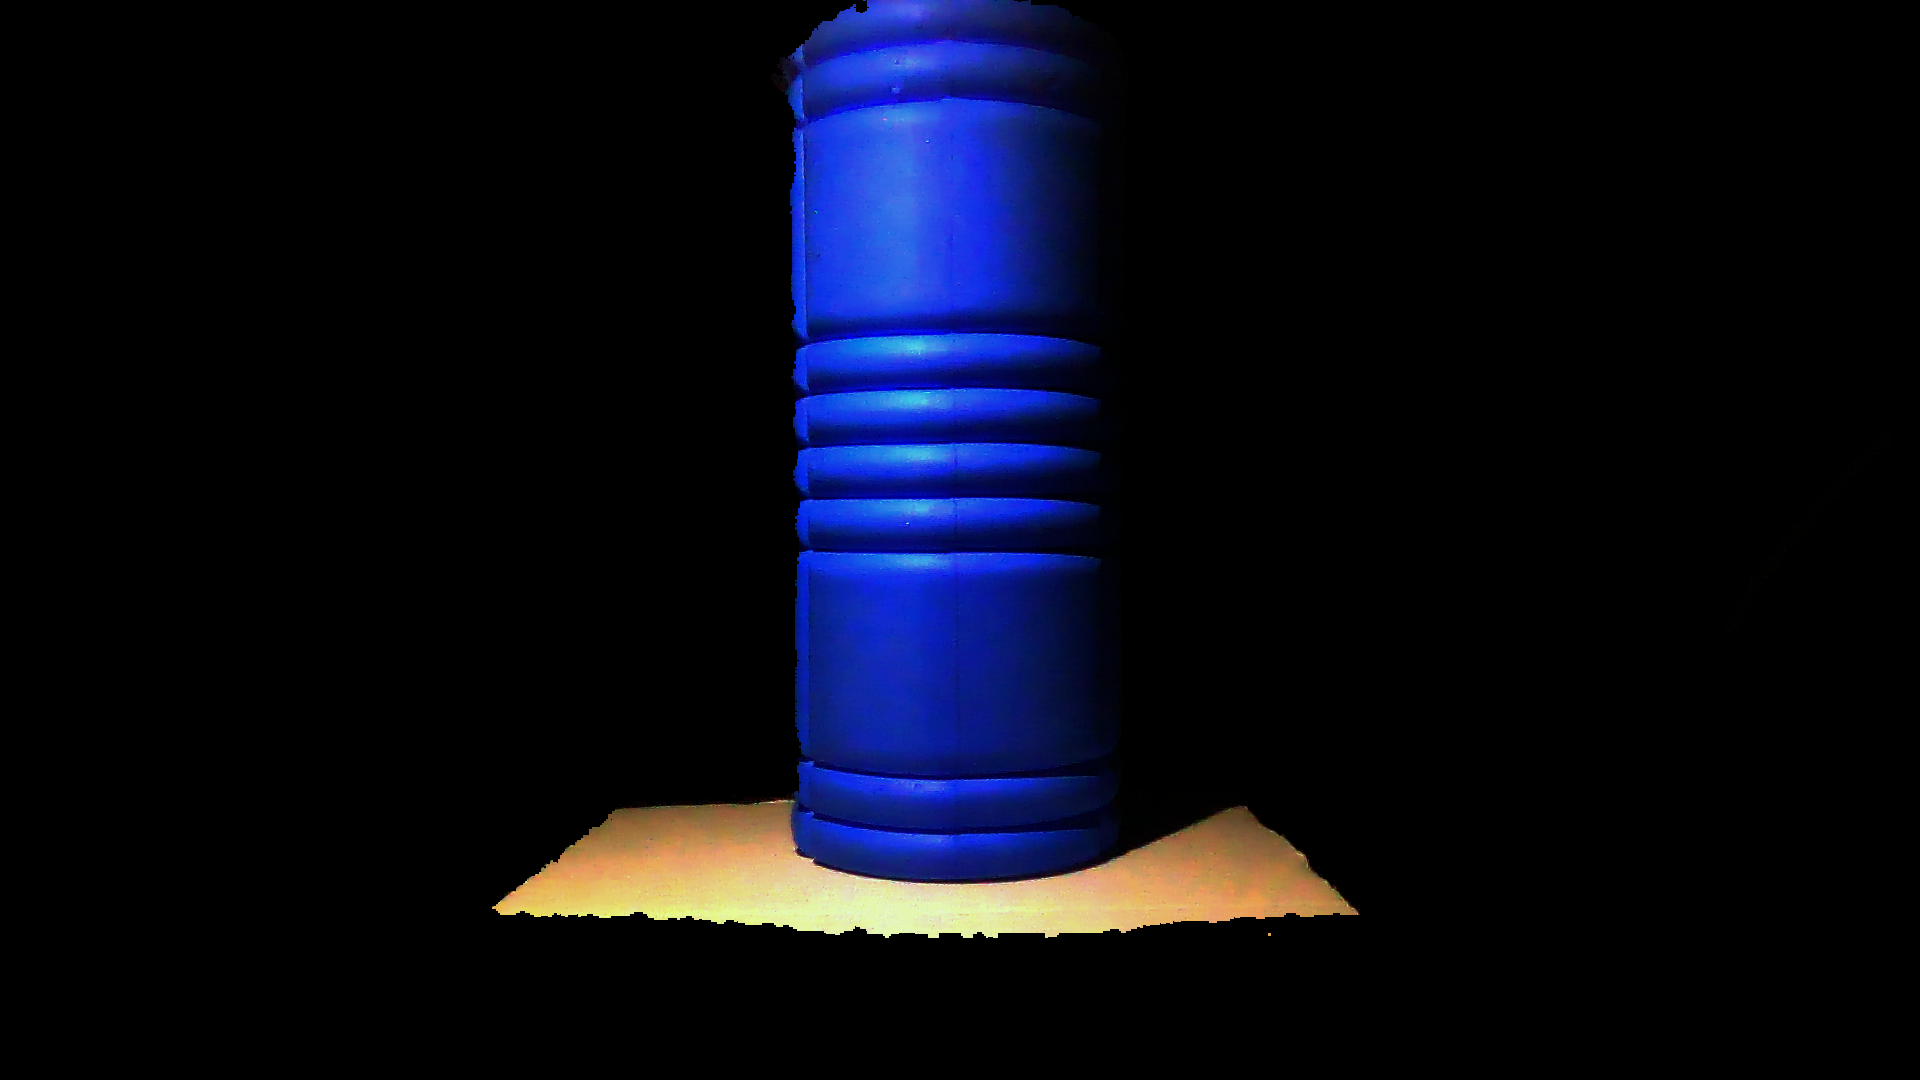
\includegraphics[width=8cm]{roller_img_sample}	
\caption{Some sample raw frames retrieved from the intel L515.}
\end{figure}

{\small
\bibliographystyle{ieee_fullname}
\bibliography{egbib}
}

\end{document}
